\begin{minipage}{0.5\textwidth}
    The LT3741  is both voltage  regulated and current  regulated. The voltage
    divider  $R_{11}  \parallel  R_2$  (Figure  \ref{fig:circuit:buck:uset}  )
    allows for  the measurement of  the output  voltage, and a  shunt resistor
    $R_4$ allows  for the exact monitoring  of the current going  through coil
    $L_1$. The value  for resistor $R_4$ (fold-out  overview schematic, Figure
    \ref{fig:circuit:buck}) was chosen so that the maximum outoing current can
    be \SI{5}{\ampere}.

    Monitoring the  current is extremely  important for  a setup in  which the
    outgoing  voltage can  be constantly  changing. It allows  to predict  the
    behavior  of  the output  voltage,  thus  enabling  the device  to  better
    suppress spikes in  output voltage and spikes in the  current through coil
    $L_1$ (Figure \ref{fig:circuit:buck} on fold-out).

    Furthermore,  a  controller   regulated  by  current  can   also  be  used
    as  a  constant  current  source. This  property  is  of  importance  when
    the  operating  point   is  in  the  steeper  part  of   the  PV  module's
    I-V-curve  (where   small  changes   in  voltage   can  lead   to  drastic
    changes  in current,  see section  \ref{subsec:regimplementation} on  page
    \pageref{subsec:regimplementation}).

\end{minipage}
\begin{minipage}{0.5\textwidth}
    \center
    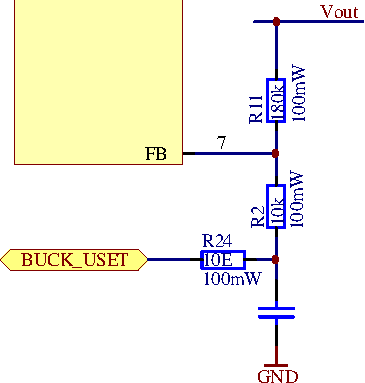
\includegraphics[width=.85\textwidth]{images/circuit/buck-uset.pdf}
    %\captionof{figure}{Regulation of output voltage by changing the reference voltage in the feedback loop via an analog reference voltage between \SI{0}{\volt} and \SI{1.21}{\volt}}
    \captionof{figure}{Circuit for regulating output voltage by changing reference voltage via $BUCK\_USET$ from the first DAC}
    \label{fig:circuit:buck:uset}
\end{minipage}

\begin{minipage}{.4\textwidth}
    The  values for  the feedback  resistors  $R_2$ and  $R_{11}$ were  chosen
    according to formula  \ref{eq:circuit:buck:feedback_resistors} so that the
    output voltage does not exceed \SI{23}{\volt}.
\end{minipage}
\begin{minipage}{.6\textwidth}
    \begin{equation}
        V_{out} = \SI{1.21}{\volt} \left( 1 + \frac{R_{11}}{R_2} \right)
        \label{eq:circuit:buck:feedback_resistors}
    \end{equation}
\end{minipage}

\begin{minipage}{.40\textwidth}
    By  increasing  $BUCK\_USET$  in formula  \ref{eq:circuit:buck:uset},  the
    outgoing  voltage can  then be  modified as  needed.  $BUCK\_USET$  is the
    analog voltage  coming from the  first DAC. The associated circuit  can be
    found in Figure \ref{fig:circuit:buck:uset}.
\end{minipage}
\begin{minipage}{.60\textwidth}
    \begin{equation}
        V_{out} = (\SI{1.21}{\volt} - BUCK\_USET) \cdot \frac{R_{11} + R_2}{R_2}
        \label{eq:circuit:buck:uset}
    \end{equation}
\end{minipage}


\begin{minipage}{.50\textwidth}
    In a manner analogous to regulating the output voltage, the maximum output
    current can  also be  controlled.  By applying  an analog  voltage between
    \SI{0}{\volt}  and \SI{1.5}{\volt}  at  input \code{CTRL1}  of the  LT3741
    controller,  the maximum  average  current going  through  coil $L_1$  and
    therefore the maximum output current can be directly controlled.

    The     corresponding    circuit     can     be     found    in     Figure
    \ref{fig:circuit:buck:iset}.  The maximum average  output current $I_o$ is
    calculated using equation \ref{eq:circuit:buck:output_current}.

    For  this, $V_{CTRL1}$  is the  analog reference  voltage coming  from the
    second DAC and  $R_4$ is the shunt  resistor (\SI{10}{\milli\ohm}, visible
    on the fold-out in Figure \ref{fig:circuit:buck}).

\end{minipage}
\begin{minipage}{.50\textwidth}
    \center
    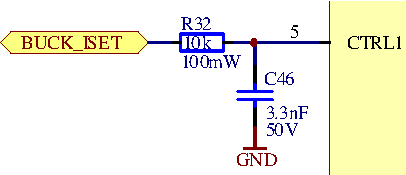
\includegraphics[width=.9\textwidth]{images/circuit/buck-iset.pdf}
    \captionof{figure}{Setting the maximum output current via reference voltage between \SI{0}{\volt} and \SI{1.5}{\volt}}
    \label{fig:circuit:buck:iset}
    \begin{equation}
        I_o = \frac{V_{CTRL1}}{30 \cdot R_4}
        \label{eq:circuit:buck:output_current}
    \end{equation}
\end{minipage}


\begin{minipage}{.50\textwidth}
    For  the  microcontroller  to  generate  appropriate  reference  voltages,
    it  needs  to   measure  both  output  voltage   and  output  current. The
    output    voltage   is    measured    with   the    circuit   in    Figure
    \ref{fig:circuit:buck:umeas}. The  values   for  resistors   $R_{12}$  and
    $R_{15}$  are such  that  voltage  $BUCK\_UMEAS$ is  scaled  to the  range
    between \SI{0}{\volt} and \SI{1.5}{\volt}.

    The  output   current  is  measured  differentially   via  shunt  resistor
    $R_5$. The    corresponding   circuit    can    be    seeen   in    Figure
    \ref{fig:circuit:buck:imeas}.

\end{minipage}
\begin{minipage}{.50\textwidth}
    \center
    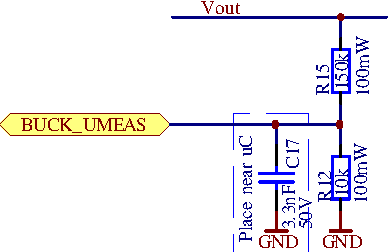
\includegraphics[width=.8\textwidth]{images/circuit/buck-umeas.pdf}
    \captionof{figure}{Measuring output voltage}
    \label{fig:circuit:buck:umeas}
\end{minipage}

\begin{figure}[th!]
    \center
    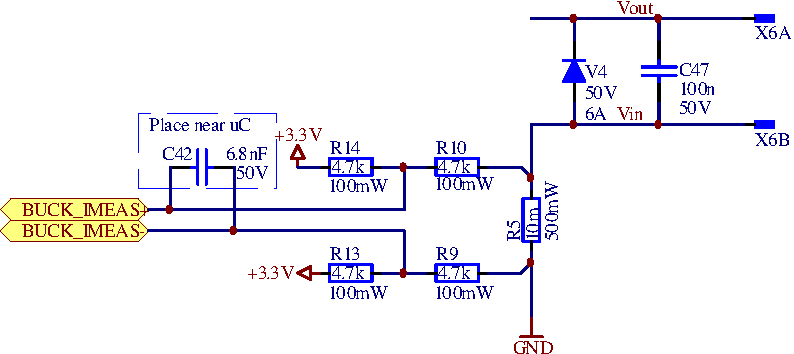
\includegraphics[width=.85\textwidth]{images/circuit/buck-imeas.pdf}
    \caption{Measuring output current}
    \label{fig:circuit:buck:imeas}
\end{figure}

\begin{minipage}{.50\textwidth}
A  particular problem  for this  measurement  is that  resistors $R_{10}$  and
$R_{14}$ cause a  bias current to flow through the  shunt resistor $R_5$, thus
leading  to an  offset $V_{offset}$  of the  measured voltage  over $R_5$,  as
calculated by equation \ref{eq:circuit:buck:shunt_offset}.
\end{minipage}
\begin{minipage}{.50\textwidth}
    \begin{equation}
        V_{offset} = \frac{ \SI{3.3}{\volt} \cdot R_5 }{ R_{14} + R_{10} + R_5 }
        \label{eq:circuit:buck:shunt_offset}
    \end{equation}
\end{minipage}

\begin{minipage}{.50\textwidth}
    Since  the  ADC  has  a  resolution   of  12  bits  and  a  reference  voltage
    of   \SI{3.3}{\volt},   one  voltage   increment   amounts   to  $V_{step}   =
    \frac{\SI{3.3}{\volt}}{2^{12}} = \SI{806}{\micro\volt}$

    Resistors $R_9$,  $R_{10}$, $R_{13}$  and $R_{14}$ should  be as  small as
    possible in order to reduce disturbances  in the traces, while at the same
    time being large enough for $V_{offset}$ to be smaller than $V_{step}$. In
    order for the ADC's holding time not to be too long (which happens roughly
    at $\geq \SI{5}{\kilo\ohm}$), they should however also not be too large.

    Thus, we can now  solve for the four resistor values,  as seen in on the right.
\end{minipage}
\begin{minipage}{.50\textwidth}

    %Equations \ref{eq:circuit:buck:shunt_offset} \ref{eq:circuit:buck:adc_step} can now
    %be solved for the four resistor values:

    \begin{align*}
                              V_{step} &\geq V_{offset} \\
        \frac{\SI{3.3}{\volt}}{2^{12}} &\geq \SI{3.3}{\volt} \cdot \frac{R_5}{R_x + R_5} \\
                      \frac{1}{2^{12}} &\geq \frac{R_5}{R_x + R_5} \\
                                   R_x &\geq \left( 2^{12} - 1 \right) \cdot R_5 \\
        \label{eq:solvethings}
    \end{align*}
    \hspace*{2em}whereby $\frac{R_x}{2} =  R_{9} = R_{10} = R_{13} =  R_{14}$.
\end{minipage}

This yields as its result $\frac{R_x}{2} \approx \SI{22}{\ohm}$.


\begin{minipage}{.50\textwidth}
    A  further  limitation,  especially  for  smaller  resistors,  is  not  to
    dissipate  too  much  power. For  this   reason,  the  resistors  will  be
    dimensioned  slightly   higher  at  \SI{270}{\ohm}. Thus,   the  resulting
    dissipated  power for  all  four resistors  is  calcualted using  equation
    \ref{eq:P_loss}.
\end{minipage}
\begin{minipage}{.50\textwidth}
    \begin{equation} \label{eq:P_loss}
        P_{loss} \approx \frac{\left(\SI{3.3}{\volt}\right)^2}{2\cdot \SI{270}{\ohm}} \approx \SI{20}{\milli\watt}
    \end{equation}
\end{minipage}

The measured  voltage at the  shunt resistor is comparatively  small. For this
reason, we use the microcontroller's integrated pre-amplifier (PGA), which can
attain a gain  of up to factor  64. The amplified signal is then  passed on to
the internal differential ADC.
